%======================================================================
%   Zak Webb
%   Ph. D. Thesis
%   Department of Physics and Astronomy
%   University of Waterloo
% 
%   Scattering Gadgets
%======================================================================


\documentclass[../thesis-main/thesis-main]{subfiles}
\begin{document}

\chapter{Scattering gadgets}
\label{chap:scattering_gadgets}

At this point, we have from \chap{scattering_on_graphs} the basic framework used or scattering on graphs.  However, everything from the chapter is a theoretical construction, where we are given a graph with a particular scattering behavior; nothing was mentioned about finding such graphs.  This chapter is dedicated to this idea of finding gadgets with particular scattering behavior, or showing that they cannot exist.


%\subsection{Momentum dependent actions}
%
%While the NAND tree algorithm gives a good example of how graph scattering can work as an algorithmic tool, in that the scattering evaluates a binary function, the scattering behavior was relatively simple: a particle transmits or reflects.  However, we can use similar ideas in order to have nontrivial scattering behavior, by creating graphs that have different behaviors at different momenta, or that perfectly transmits to some subset of the attached paths (i.e., a generalization of perfect transmission to multiple semi-infinite paths).
%
%\todo{Should I include schematic pictures of these gadgets?  I'm not sure if that would improve readability}
%
%%%%%%%%%%%%%%%%%%%%%%%%%%%%%%%%%%%%%%%%%%%%%%%%%%%%%%%%%%%%%%%%%%
%
%\subsubsection{R/T gadgets}
%
%The easiest thing we could hope for is the same behavior as in the NAND tree algorithm, with two attached paths and at some fixed momenta the wavepacket either completely transmits, or it completely reflects.  However, we will utilize a single graph with several different momenta.
%
%In particular, these reflection/transmission (R/T) gadgets will have two sets of momenta.   One set will have perfect transmission, while the other will have perfect reflection.  While these gadgets have relatively simple scattering behavior, they can be used to filter particular momenta, or as building blocks in more complicated gadgets.  Additionally, the simple behavior will allow us to show that certain scattering behaviors are not possible.
%
%%%%%%%%%%%%%%%%%%%%%%%%%%%%%%%%%%%%%%%%%%%%%%%%%%%%%%%%%%%%%%%%%%
%
%\subsubsection{Momentum Switches}
%
%We can generalize the idea of R/T gadgets to multiple semi-infinite paths, so that the gadget has a kind of routing behavior.  In particular, we can attempt to construct graphs with three attached semi-infinite paths, in which when a wavepacket is incident along one particular path, it either perfectly transmits to the second path, or it perfectly transmits to the third path, depending on the incident momenta.  In this way, we construct something like a momentum dependent railroad switch, sending different wavepackets to different locations.
%
%These momentum switches are extremely useful, as they will allow us to construct much more interesting momentum dependent behavior.  By using two of these gadgets in series (with the paths 2 and 3 connected to each other), we can then place a single obstacle along only one of the paths.  Since only those momenta that travel along that particular path are incident on the additional obstacle, we can use this to do something like applying a momentum dependent phase.
%
%%%%%%%%%%%%%%%%%%%%%%%%%%%%%%%%%%%%%%%%%%%%%%%%%%%%%%%%%%%%%%%%%%
%
%\subsection{Encoded unitary}
%
%While the above two gadgets can be thought to have one input but two output paths, we can generalize this idea to having multiple input paths.  In particular, if we have two input and two output paths, we can encode a logical qubit in a dual-rail encoding (i.e., one path corresponds to a state $\ket{0}$, while the other corresponds to a state $\ket{1}$).  If we can ensure that wavepackets incident along the input paths always transmit to the output paths, we can think of this as applying a unitary gate to the encoded qubit.
%
%In particular, by constructing a gadget whose $S$-matrix at a particular momentum is block diagonal, with two zero blocks along the diagonal, we have that a wavepacket at that momenta always transmits from the input to the output vertices.  Additionally, as the $S$-matrix is itself unitary, we have that the $2\times2$ block matrix that corresponds to the transmitted amplitudes is also unitary, and thus we have applied a unitary operation to the encoded qubit.  
%
%
%%%%%%%%%%%%%%%%%%%%%%%%%%%%%%%%%%%%%%%%%%%%%%%%%%%%%%%%%%%%%%%%%
%  Constructing graphs
%%%%%%%%%%%%%%%%%%%%%%%%%%%%%%%%%%%%%%%%%%%%%%%%%%%%%%%%%%%%%%%%%

\section{Constructing graphs with particular scattering behavior}

While we have shown that the scattering behavior of some given graph is easy to compute, finding graphs with a given behavior is much more difficult.  We don't even know whether such an operation is decidable, and thus finding an algorithm to construct a graph with a given $S$-matrix seems unlikely.  However, there are specific behaviors at particular momenta in which constructions are known, and exhaustive searches of small sized graphs have yielded graphs with nice scattering properties.  

In particular, Andrew Childs found several gadgets in his paper proving the universality of quantum walks \cite{Chi09}.  After this result, Blumer, Underwood and Feder \cite{BUF11} performed an exhaustive search over all graphs with at most 9 vertices, finding those graphs that implement an encoded unitary at several momenta of interest.  Childs, Gosset, and Webb then constructed several gadgets in \cite{MPQW}.  This section is mainly based on \cite{MomSwitches}, a paper by Chlids, Gosset, Nagaj, Raha, and Webb, as it gives explicit constructions for gadgets with particular behavior.

%%%%%%%%%%%%%%%%%%%%%%%%%%%%%%%%%%%%%%%%%%%%%%%%%%%%%%%%%%%%%%%%%

\subsection{R/T gadgets}\label{sec:rt_gadgets}
 
Perhaps the most simple behavior, and the one that will for which we will have the easiest time finding a solution, are two-terminal gadgets that either perfectly reflect at some particular momenta, or perfectly transmit.  These R/T gadgets can be thought of as a proof-of-principle for constructing gadgets, but they also have uses of their own.

This problem is still rather complicated when we work with arbirtary graphs with two terminal vertices, things become much simpler if we work with a graph attached to an infinite path via a single vertex.  In this case, we can determine exactly when the gadget will lead to perfect reflection, and when it will lead to perfect transmission.

\begin{figure}
  \centering
  \tikzsetnextfilename{SG_reversal_orig}
  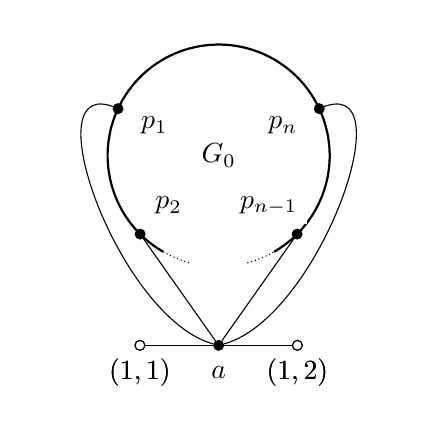
\begin{tikzpicture}[
  label distance=-5.5pt,
  thin,
  vertex/.style={circle,draw=black,fill=black,inner sep=1.25pt,
    minimum size =0mm},
  attach/.style={circle,draw=black,fill=white,inner sep=1.25pt,
    minimum size =0mm},
  dots/.style={circle,fill=black,inner sep=.5pt,
    minimum size= 0pt}]

% Path and Labels    
  \draw (-1,-2.41) -- (1,-2.41);
  
  \foreach \x /\n in {-1/ 1, 1/2}{
    \node at (\x,-2.41) [attach] {};
    \node at (\x,-2.75) {$(1,\n)$};
  }
    
  \node (a) at (0,-2.41) [vertex] {};
  \node at (0,-2.75) {$a$};
  
  \foreach \x /\n in {-1/ 1, 1/2}{
    \node at (\x,-2.41) [attach] {};
    \node at (\x,-2.75) {$(1,\n)$};
  }
  
% Graph  
  \draw[thick] (240:1.41) arc (240:-60:1.41);
  \draw[densely dotted] (240:1.41)  arc (240:255:1.41);
  \draw[densely dotted] (285:1.41)  arc (285:300:1.41);
  
  \foreach \i / \n /\t in {25 / n/ 15, 155 / 1/ 165, 225/ 2 / 120, 315 / {n-1}/60}{
    \node at (\i : .9) [rectangle,fill=white] {$p_\n$};
    \node at (\i : 1.41) [vertex] {};
  }
  \node at (0,0) [rectangle,fill=white] {$G_0$};

% Attaching Edges
  \foreach \i /\t in {25/15, 155/165}{
    \draw (\i:1.41) to[out=\i,in=\t] (a);
  }
  
  \foreach \i \in in {225,315}{
    \draw (\i:1.41) to (a);
  }

\end{tikzpicture}
  \caption[A type 1 R/T gadget]{A type 1 R/T gadget.  Vertices of $G_0$ that are not part of the periphery $P = \{p_1,\ldots,p_n\}$ are not shown.}
  \label{fig:reversal_orig}
\end{figure}

Along these lines, we will investigate the scattering behavior of graphs where $\widehat{G}$ is of the form found in \fig{reversal_orig}.  While we still have that $\widehat{G}$ is of the form described in \sec{general_graphs}, the graph $G$ with the semi-infinite paths is that of a infinite path, with the graph $G_0$ attached to the vertex $a$.  As such, the graph that will be of more interest is the graph $G_0$ consisting of those vertices other than those along the infinite path.   We will label those vertices $p_i\in V(G_0)$ connected to the vertex $a$ as \emph{periphery} vertices, and we will label the set of periphery vertices as $P$.  In the special case that $|P| = 1$, or that a single vertex of $G_0$ is connected to $a$, we will call the gadget a type 2 R/T gadget (see \fig{RT_path} for an example of a type 2 R/T gadget).

For a given R/T gadget $\widehat{G}$, those momenta for which perfect reflection occurs shall be collected in the \emph{reflection set} which shall be denoted $\mathcal{R}$.  Similarly, those momenta for which perfect transmission occurs shall be collected in the \emph{transmission set} which shall be label $\mathcal{T}$. Note that these two sets have empty intersection, and that there isn't any nice relationship between them.

Let us now examine the scattering eigenstates for the graph $\widehat{G}$.  For any scattering state $\ket{\scat_{1} (k)}$, by examining the eigenvalue equation at vertices $(1,1)$ and $(1,2)$ we see that the amplitude at vertex $a$ satisfies
\begin{equation}
  \langle{a}\ket{\scat_{1} (k)} = 1 + R(k) = T(k).
\end{equation}
Thus perfect reflection at momentum $k$ occurs if and only if $R(k)=-1$ and $\langle{a}\ket{\scat_{1} (k)}=0$, while perfect transmission occurs if and only if $T(k)=1$ and $\langle{a}\ket{\scat_{1} (k)}=1$. Using this fact, we now derive conditions on the graph $G_0$ that determine when perfect transmission and reflection occur.

For any type 1 R/T gadget, we have necessary and sufficient conditions for momentum $k$ to be in the reflection set: $G_0$ should have an eigenvector for which the sum of amplitudes on the periphery is nonzero.
\begin{lemma}
Let $\widehat{G}$ be a type 1 R/T gadget. A momentum $k\in (-\pi,0)$ is in the reflection set $\mathcal{R}$ if and only if $G_0$ has an eigenvector $\ket{\chi_k}$ with eigenvalue $2\cos(k)$ satisfying
\begin{equation}
  \sum_{i=1}^{n} \braket{p_i}{\chi_k} \neq 0. \label{eq:sum_condition}
\end{equation}
\label{lem:reflect_reqs}
\end{lemma}

\begin{proof}
Let us first suppose that $\widehat{G}$ has perfect reflection at momentum $k$, i.e., $R(k)=-1$ and $\langle{a}\ket{\scat_{1} (k)}=0$. As $\langle{(1,1)}\ket{\scat_1(k)} = e^{-ik} - e^{ik}\neq 0$ and $\langle{(1,2)}\ket{\scat_1(k)}=0$, to satisfy the eigenvalue equation at vertex $a$, we have
\begin{equation}
  \sum_{j=1}^{n} \langle{p_j}\ket{\scat_1(k)} = e^{ik} - e^{-ik} \neq 0.
\end{equation}
Further, since $G_0$ only connects to vertex $a$ and the amplitude at this vertex is zero, the restriction of $\ket{\scat_1(k)}$ to $G_0$ must be an eigenvector of $G_0$ with eigenvalue $2\cos(k)$. Hence the condition is necessary for perfect reflection. 
 
Next suppose that $G_0$ has an eigenvector $\ket{\chi_k}$ with eigenvalue $2\cos(k)$ satisfying \eq{sum_condition}, with the sum equal to some nonzero constant $c$. Define a scattering state $\ket{\psi_k}$ on the Hilbert space of the full graph $G$ with amplitudes
\begin{equation}
  \braket{v}{\psi_k} = \frac{e^{ik} - e^{-ik}}{c} \braket{v}{\chi_k}
\end{equation}
for all $v \in V(G_0)$, $\braket{a}{\psi_k}=0$, and 
\begin{equation}
 \braket{(x,j)}{\psi_k}=\begin{cases} e^{-ikx}-e^{ikx} & j=1\\
0 & j=2
\end{cases}
\end{equation}
for all $x \in \posint$.

We claim that $\ket{\psi_k}$ is an eigenvector of $G$ with eigenvalue $2 \cos(k)$.  The state clearly satisfies the eigenvalue equation on the semi-infinite paths since it is a linear combination of states with momentum $\pm k$.  At vertices of $G_0$, the state is proportional to an eigenvector of $G_0$, and since the state has no amplitude at $a$, the eigenvalue equation is also satisfied at these vertices.  It remains to see that the eigenvalue equation is satisfied at $a$, but this follows immediately by a simple calculation.

Since $\ket{\psi_k}$ has the form of a scattering state with perfect reflection, we see that $R(k)=-1$ and $T(k)=0$ as claimed.
\end{proof}

In a similar manner, the following lemma gives a sufficient condition for a momentum $k$ to be in the transmission set (which is also necessary for type 2 gadgets).  Let $g_0$ denote the induced subgraph on $V(G_0)\setminus P$ where $P = \{p_i\colon i\in [n]\}$ is the periphery.

\begin{lemma}\label{lem:transmit_reqs}
Let $\widehat{G}$ be a type 1 R/T gadget and let $k\in (-\pi,0)$. Suppose $\ket{\xi_k}$ is an eigenvector of $g_0$ with eigenvalue $2\cos{k}$ and with the additional property that, for all $i \in [n]$,
\begin{equation}
\label{eq:trans_cond}
  \sum_{\substack{v \in V(g_0): \\ (v,p_i)\in E(G_0)}} \braket{v}{\xi_k} = c \neq 0 
\end{equation}
for some constant $c$ that does not depend on $i$. Then $k$ is in the transmission set $\mathcal{T}$. If $\hat{G}$ is a type 2 R/T gadget, then this condition is also necessary.
\end{lemma}

\begin{proof}
If $g_0$ has a suitable eigenvector $\ket{\xi_k}$ satisfying \eq{trans_cond}, define a scattering state $\ket{\psi_k}$ on the full graph $G$, with amplitudes $\langle a\ket{\psi_k}=1$, 
\begin{equation}
  \braket{v}{\psi_k} 
  = \begin{cases} -\frac{1}{c} \braket{v}{\xi_k} & v\in V(g_0)\\
  	0 & v \in P
\end{cases}
\label{eq:psik_c}
\end{equation}
in the graph $G_0$, and 
\begin{equation}
 \langle{(x,j)} \ket{\psi_k}=\begin{cases} e^{-ikx} & j=1\\
 e^{ikx} & j=2
\end{cases}
\end{equation}
for $x \in \posint$.  As in the proof of \lem{reflect_reqs}, the state $\ket{\psi_k}$ is clearly satisfies the eigenvalue equation (with eigenvalue $2\cos(k)$) at vertices on the semi-infinite paths and vertices of $g_0$.  The factor of $-\frac{1}{c}$ in \eq{psik_c} is chosen so that the eigenvalue condition is satisfied at vertices in $P$.  It is easy to see that the eigenvalue condition is also satisfied at $a$.

Since $\ket{\psi_k}$ is a scattering eigenvector of $G$ with eigenvalue $2\cos(k)$ and perfect transmission, we have $T(k)=1$.

Now suppose $\widehat{G}$ is a type 2 R/T gadget, with $P = \{p\}$.  Perfect transmission along with the eigenvalue equation at vertex $a$ implies
\begin{equation}
\braket{p}{\scat_1(k)} = 0,
\end{equation}
so the restriction of $\ket{\scat_1(k)}$ to $g_0$ must be an eigenvector (since $p$ is the only vertex connected to $g_0$).  The eigenvalue equation at $p$ gives
\begin{equation}
  \braket{a}{\scat_1(k)} 
  + \sum_{w \colon (w,p)\in E(G_0)} \braket{w}{\scat_1(k)} = 0 
  \quad\implies\quad
  \sum_{w \colon (w,p)\in E(G_0)} \braket{w}{\scat_1(k)} = -1.
\end{equation}
Hence the restriction of $\ket{\scat_1(k)}$ to $V(g_0)$ is an eigenvector of the induced subgraph, with the additional property that the sum of the amplitudes at vertices connected to $p$ is nonzero.
\end{proof}

With these two lemmas, if we can guarantee the form of the eigenstates for the graph $G_0$, we can guarantee certain momenta to be in either the reflection or the transmission set.


%%%%%%%%%%
\subsubsection{Explicit constructions}\label{sec:rt_ex}

While the two lemmas do give a nice abstract explanation for the construction of R/T gadgets, it doesn't provide us with a concrete example. As such, let us look at two simple graphs and examine when they satisfy the conditions of the lemmas.

As a first example, suppose $G_0$ is a finite path of length $l_1+l_2-2$ connected to $a$ at the $l_1$th vertex, as shown in \fig{RT_path}.  As this is a type 2 R/T gadget, we can then determine the reflection and transmission sets as a function of $l_1$ and $l_2$.


%%%%%%%%%
\begin{figure}
  \centering
  \tikzsetnextfilename{SG_RT_path}
  \begin{tikzpicture}[
  thin,
  vertex/.style={circle,draw=black,fill=black,inner sep=1.25pt,
    minimum size =0mm},
  attach/.style={circle,draw=black,fill=white,inner sep=1.25pt,
    minimum size =0mm},
  dots/.style={circle,fill=black,inner sep=.5pt,
    minimum size= 0pt}]
    
    \draw (-1,-1) -- (1,-1);
    \draw (0,0) -- (0,-1);
    
    \node[attach,label=270:{$(1,1)$}] at (-1,-1) {};
    \node[attach,label=270:{$(1,2)$}] at (1,-1) {};
    \node[vertex,label={[label distance=.25*\baselineskip]270:{$ a $}},] at (0,-1) {};
    \node[vertex] at (0,0) {};
    
    % left branch
    \draw (0,0) -- (135:1.5);
    \draw[densely dotted] (135:1.5) -- (135: 2.25);
    
    \draw[densely dotted] (135:2.75) -- (135:3.5);
    \draw (135:3.5) -- (135:5);
    
    \foreach \r in {1,5,4}{
      \node[vertex] at (135:\r) {};
    }
    

    \foreach \n /\p in {1/5,2/4,{l_1-1}/1}{
      \node at (135:\p) [label={225:$\n$}] {};
    }
    
    
    % right branch
    \draw (0,0) -- (45:1.5);
    \draw[densely dotted] (45:1.5) -- (45: 2.25);
    
    \draw[densely dotted] (45:3.75) -- (45:4.5);
    \draw (45:4.5) -- (45:6);
        
    \foreach \r in {1,6,5}{
      \node[vertex] at (45:\r) {};
    }    
    
    
    \foreach \n /\p in {{l_1}/0,{l_1+1}/1,{l_1+l_2-2}/5,{l_1+l_2-1}/6}{
      \node at (45:\p)[label=315:{$\n$}]{};
    }    

\end{tikzpicture}
  \caption[An R/T gadget from a path]{An R/T gadget built from a path of length $l_1+l_2-2$. }
  \label{fig:RT_path}
\end{figure}


Using \lem{reflect_reqs}, we see that perfect reflection occurs at momentum $k\in (-\pi,0)$ if and only if the path has an eigenvector with eigenvalue $2\cos(k)$ with non-zero amplitude on vertex $l_1$.  Recall that the path of length $L$ (where the length of a path is its number of edges) has eigenvectors $|\psi_j\rangle$ for $j\in [L+1]$ given by
\begin{equation}
  \langle x | \psi_j \rangle = \sin\left(\frac{ \pi j x}{L+2}\right)\label{eq:vecs_line}
\end{equation}
with eigenvalues $\lambda_j = 2 \cos(\pi j/(L+2))$.  Hence
\begin{equation}
  \mathcal{R}_{\mathrm{path}} = \left\{ -\frac{\pi j}{l_1 + l_2} \colon j\in [l_1 + l_2 - 1] \text{ and } \frac{jl_1}{l_1+l_2} \not\in \ZZ\right\}.
\end{equation}

To characterize the momenta at which perfect transmission occurs, consider the induced subgraph obtained by removing the $l_1$th vertex from the path of length $l_1+l_2-2$ (a path of length $l_1-2$ and a path of length $l_2-2$). We can choose bases for the eigenspaces of this induced subgraph so that each eigenvector has all of its support on one of the two paths, and has nonzero amplitude on only one of the vertices $l_1-1$ or $l_1+1$. Thus \lem{transmit_reqs} implies that $\widehat{G}$ perfectly transmits for all momenta in the set
\begin{equation}
  \mathcal{T}_{\mathrm{path}} = \left\{- \frac{\pi j}{l_1} \colon j\in [l_1-1]\right\} \cup \left\{-\frac{\pi j}{l_2 } \colon j \in [l_2-1]\right\}.
\end{equation}

As an explicit example, if we set $l_1 = l_2 = 2$, we get $\mathcal{T}_{\mathrm{path}} = \{-\frac{\pi}{2}\}$ and $\mathcal{R}_{\mathrm{path}} = \{-\frac{\pi}{4}, -\frac{3\pi}{4}\}$.


Now let us suppose $G_0$ is a cycle of length $r$. Labeling the vertices by $x \in [r]$, where $x=r$ is the vertex attached to the path (as shown in \fig{RT_cycle}), the eigenvectors of the $r$-cycle are
\begin{equation}
  \langle x | \phi_m\rangle = e^{{2 \pi i x m}/{r}}
\end{equation}
with eigenvalue $2 \cos(2 \pi m/r)$, where $m\in [r]$. For each momentum $k=-2 \pi m/r \in (-\pi,0)$, there is an eigenvector with nonzero amplitude on the vertex $r$ (i.e., $\langle r | \phi_m\rangle\neq 0$), so \lem{reflect_reqs} implies that perfect reflection occurs at each momentum in the set
\begin{equation}
  \mathcal{R}_{\mathrm{cycle}} = \left\{ -\frac{\pi j}{r} \colon \text{$j$ is even and $j\in [r-1]$}\right\}.
\end{equation}


%%%%%%%%%
\begin{figure}
  \centering
  \tikzsetnextfilename{SG_RT_cycle}
  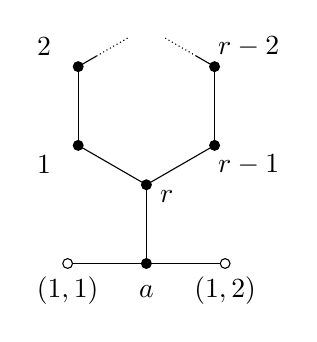
\begin{tikzpicture}[
  thin,
  vertex/.style={circle,draw=black,fill=black,inner sep=1.25pt,
    minimum size =0mm},
  attach/.style={circle,draw=black,fill=white,inner sep=1.25pt,
    minimum size =0mm},
  dots/.style={circle,fill=black,inner sep=.5pt,
    minimum size= 0pt}]
    \draw (-1,-2) -- (1,-2);
    \draw (0,-2) -- (0,-1);
    
    \node[attach] at (-1,-2) {};
    \node at (-1,-2.35) {$(1,1)$};
    \node[attach] at (1,-2) {};
    \node at (1,-2.35) {$(1,2)$};
    \node[vertex] at (0,-2) {};
    \node at (0,-2.35) {$a$};
    
    \foreach \t in {150, 210, 270, 330, 30}{
      \node[vertex] at (\t: 1) {};
    }
    
    \foreach \t in {210, 270, 330, 30}{
      \draw (\t:1) -- (\t - 60:1);
    }
    
    \draw (150:1) -- (135:.897);
    \draw (30:1) -- (45:.897);
    
    \draw[densely dotted] (45:.897) -- (75:.897);
    \draw[densely dotted] (135:.897) -- (105:.897);
    
    \foreach \t / \n in {210 / 1, 150 / 2, 30 / {r-2}, -30 / {r-1}}{
      \node at (\t:1.5) {$\n$};
    }
    
    \node at (.26,-1.15) {$r$};
  
\end{tikzpicture}
  \caption[An R/T gadget from a cycle]{An R/T gadget built from an $r$-cycle.}
  \label{fig:RT_cycle}
\end{figure}


To see which momenta perfectly transmit, we use \lem{transmit_reqs}. Consider the induced subgraph obtained by removing vertex $r$. This subgraph is a path of length $r-2$ and has eigenvalues $2\cos(\pi m/r)$ for $m \in [r-1]$ as discussed in the previous section. Using the expression \eq{vecs_line} for the eigenvectors, we see that the sum of the amplitudes on the two ends is nonzero for odd values of $m$.  Perfect transmission occurs for each of the corresponding momenta:  
\begin{equation}
  \mathcal{T}_{\mathrm{cycle}} = \left\{ -\frac{\pi j}{r} \colon \text{$j$ is odd and $j\in [r-1]$}\right\}.
\end{equation}

For example, the $4$-cycle (i.e., square) has $\mathcal{T}_{\mathrm{cycle}} = \{-\frac{\pi}{4},-\frac{3\pi}{4}\}$ and $\mathcal{R}_{\mathrm{cycle}} = \{-\frac{\pi}{2}\}$.  

%%%%%%%%%%%%%%%%%%%%%%%%%%%%%%%%%%%%%%
\subsubsection{Reversing reflection and transmission sets}\label{sec:reversal}

With these explicit examples of R/T gadgets, it will be useful to know how to interchange the reflection and transmission set.  Namely, if we have one gadget that transmits all momenta in $\mathcal{T}$ and reflects all momenta in $\mathcal{R}$, it will be useful to also have a gadget that reflects all momenta in $\mathcal{T}$ and transmits all momenta in $\mathcal{R}$.  Basically, we will be able to use these two gadgets together to construct gadgets with more interesting scattering behavior.

In particular, let $\widehat{G}$ be a type 2 R/T gadget, as seen in \fig{reversalRT}, and assume that it has a reflection set $\mathcal{R}$ and a transmission set $\mathcal{T}$.  We will construct a type 1 R/T gadget $\widehat{G}^{\leftrightarrow}$ with reflection set $\mathcal{R'} \supset \mathcal{T}$ and transmission set $\mathcal{T}' \supset \mathcal{R}$.  The graph $\widehat{G}^{\leftrightarrow}$ is depicted pictorially in \fig{reversal_changed}.

Explicitly, the R/T gadget $\widehat{G}^\leftrightarrow$ is obtained by taking two copies of the subgraph $g_0$ from the type 2 R/T gadget in \fig{reversalRT}, connecting both to a single additional vertex $u$, and connecting one copy of $g_0$ to the infinite path at $a$.  More concretely, for each vertex $w_j\in V(g_0)$, the graph $\widehat{G}^{\leftrightarrow}$ has two vertices $w_j^{(1)}$ and $w_j^{(2)}$, and the graph $\widehat{G}^\leftrightarrow$ inherits the edge set of $g_0$.  Additionally, for each $w_j\in V(g_0)$ connected to the periphery vertex $p$, we have that $w_j^{(i)}$ is connected to $u$, and $w_j^{(1)}$ is connected to $a$.

%%%%%%%%%%
\begin{figure}
  \centering
  \subfloat[][]{ 
    \tikzsetnextfilename{SG_reversalRT}
    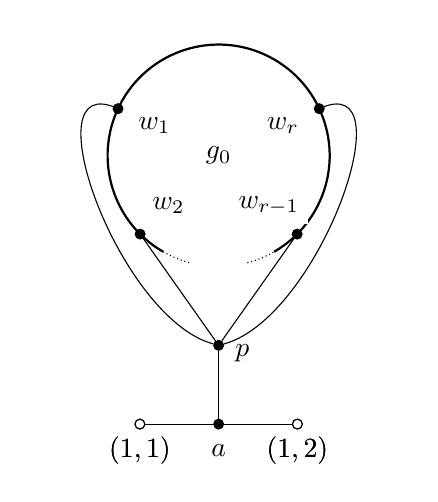
\begin{tikzpicture}[
  label distance=-5.5pt,
  thin,
  vertex/.style={circle,draw=black,fill=black,inner sep=1.25pt,
    minimum size =0mm},
  attach/.style={circle,draw=black,fill=white,inner sep=1.25pt,
    minimum size =0mm},
  dots/.style={circle,fill=black,inner sep=.5pt,
    minimum size= 0pt}]

% Path and Labels    
  \draw (-1,-3.41) -- (1,-3.41);
  
  \foreach \x /\n in {-1/ 1, 1/2}{
    \node at (\x,-3.41) [attach] {};
    \node at (\x,-3.75) {$(1,\n)$};
  }
    
  \node (a) at (0,-3.41) [vertex] {};
  \node at (0,-3.75) {$a$};
  
  \foreach \x /\n in {-1/ 1, 1/2}{
    \node at (\x,-3.41) [attach] {};
    \node at (\x,-3.75) {$(1,\n)$};
  }
  
  \node (v) at (0,-2.41) [vertex]{};
  \node at (0.3,-2.51) {$p$};
  \draw (v) to (a);
  
% Graph  
  \draw[thick] (240:1.41) arc (240:-60:1.41);
  \draw[densely dotted] (240:1.41)  arc (240:255:1.41);
  \draw[densely dotted] (285:1.41)  arc (285:300:1.41);
  
  \foreach \i / \n /\t in {25 / r/ 15, 155 / 1/ 165, 225/ 2 / 120, 315 / {r-1}/60}{
    \node at (\i : .9) [rectangle,fill=white] {$w_\n$};
    \node at (\i : 1.41) [vertex] {};
  }
  \node at (0,0) [rectangle,fill=white] {$g_0$};

% Attaching Edges
  \foreach \i /\t in {25/15, 155/165}{
    \draw (\i:1.41) to[out=\i,in=\t] (v);
  }
  
  \foreach \i \in in {225,315}{
    \draw (\i:1.41) to (v);
  }

\end{tikzpicture}
    \label{fig:reversalRT}
  }
  \qquad
  \subfloat[][]{
    \tikzsetnextfilename{SG_reversal_changed}
    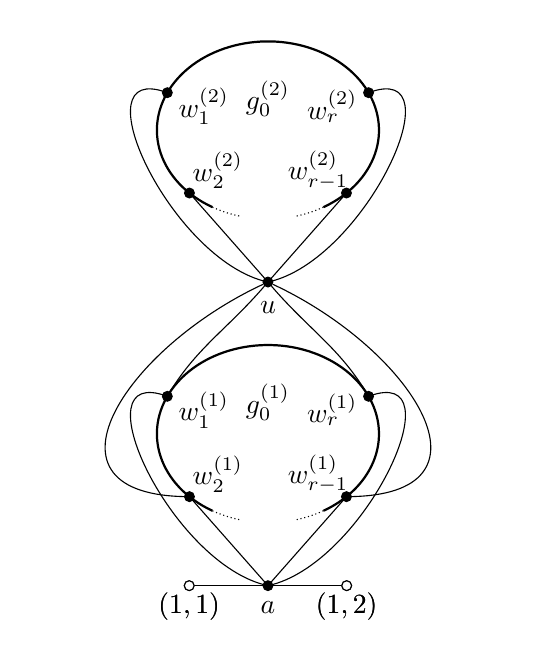
\begin{tikzpicture}[
  yscale = 0.8,
  label distance=-5.5pt,
  thin,
  vertex/.style={circle,draw=black,fill=black,inner sep=1.25pt,
    minimum size =0mm},
  attach/.style={circle,draw=black,fill=white,inner sep=1.25pt,
    minimum size =0mm},
  dots/.style={circle,fill=black,inner sep=.5pt,
    minimum size= 0pt}]

% Path and Labels    
  \draw (-1,-2.41) -- (1,-2.41);
  
  \foreach \x /\n in {-1/ 1, 1/2}{
    \node at (\x,-2.41) [attach] {};
    \node at (\x,-2.75) {$(1,\n)$};
  }
    
  \node (a) at (0,-2.41) [vertex] {};
  \node at (0,-2.75) {$a$};
  
  \foreach \x /\n in {-1/ 1, 1/2}{
    \node at (\x,-2.41) [attach] {};
    \node at (\x,-2.75) {$(1,\n)$};
  }
  
  \node (v) at (0,2.41) [vertex] {};
  \node at (0,2) {$u$};
  
% Graphs (both)

\foreach \j/\of in {1/0,2/4.82}{
\begin{scope}[yshift=\of cm]
  \foreach \i / \n /\t in {25 / r/ 15, 155 / 1/ 165, 225/ 2 / 120, 315 / {r-1}/60}{
    \node at (\i : .9) [rectangle,fill=white] {$w_\n^{(\j)}$};
    \node at (\i : 1.41) [vertex] {};
  }
  \node at (0,0.5) [rectangle,fill=white] {$g_0^{(\j)}$};
  
  \draw[thick] (240:1.41) arc (240:-60:1.41);
  \draw[densely dotted] (240:1.41)  arc (240:255:1.41);
  \draw[densely dotted] (285:1.41)  arc (285:300:1.41);

% Attaching Edges
  \foreach \i /\t in {25/15, 155/165}{
    \draw (\i:1.41) to[out=\i,in=\t] (0,-2.41);
  }
  
  \foreach \i \in in {225,315}{
    \draw (\i:1.41) to (0,-2.41);
  }
  
\end{scope}
}

  \draw (25:1.41) to [out = 115,in=-55] (v);
  \draw (155:1.41) to [out=65,in=-125] (v);
  \draw[looseness=1.5] (225:1.41) to[out=180,in=210] (v);
  \draw[looseness=1.5] (315:1.41) to[out=0,in=-30] (v);
\end{tikzpicture}
    \label{fig:reversal_changed}
   }
   \caption[Type 2 R/T Gadget and Reversal R/T gadget]{\subfig{reversalRT}  A type 2 R/T gadget, (i.e., a type 1 gadget with $|P| = 1$).  \subfig{reversal_changed}  The R/T gadget $\widehat{G}^\leftrightarrow$ reversing the reflection and transmission sets of \subfig{reversalRT}.}
   \label{fig:reversal}
\end{figure}

With this definition, we now prove that the graph $\widehat{G}^\leftrightarrow$ reverses the reflection and transmission sets of $\widehat{G}$.

\begin{lemma}\label{lem:reversal_graph}
Let $\widehat{G}$ be a type 2 R/T gadget with transmission set $\mathcal{T}$ and reflection set $\mathcal{R}$.  The type 1 R/T gadget $\widehat{G}^{\leftrightarrow}$ defined above has transmission set $\mathcal{T}' \supseteq \mathcal{R}$ and reflection set $\mathcal{R}' \supseteq \mathcal{T}$.
\end{lemma}
\begin{proof}
First consider a momentum $k\in \mathcal{T}$. Using the condition derived in \lem{transmit_reqs}, we see that $g_0$ has an eigenvector $\ket{\xi_k}$ with eigenvalue $2\cos(k)$ where the sum of the amplitudes on vertices $w_1,\ldots,w_r$ is nonzero.  Now consider the induced subgraph $G_{0}^{\leftrightarrow}$ of \fig{reversal_changed} obtained by removing vertices $(1,1)$, $(1,2)$, and $a$. This subgraph has an eigenvector $|\chi^{\leftrightarrow}_k\rangle$ with eigenvalue $2\cos(k)$ given by
\begin{equation}
  \langle v^{(i)} \ket{\chi^{\leftrightarrow}_k}= (-1)^i \langle v\ket{\xi_k} \quad \text{ and } \quad \langle{u}\ket{\chi^{\leftrightarrow}_k} = 0
\end{equation}
for all vertices $v\in V(g_0)$ and for $i \in \{1,2\}$.  The fact that $\ket{\chi_k^{\leftrightarrow}}$ is an eigenvector follows from the fact that $\ket{\xi_k}$ is an eigenvector of $g_0$.  Additionally, we have that
\begin{equation}
  \sum_{j=1}^{r} \langle{w^{(1)}_j} \ket{\chi^{\leftrightarrow}_k} = - \sum_{j=1}^{r} \langle{w_j} \ket{\xi_k} \neq 0.
\end{equation}
Using \lem{reflect_reqs}, we see that perfect reflection occurs at momentum $k$, and thus $\mathcal{T} \subseteq \mathcal{R}'$.

Next suppose $k\in \mathcal{R}$. \lem{reflect_reqs} states that $G_0$ has an eigenvector $|\chi_k\rangle$ with eigenvalue $2\cos(k)$ such that $\langle p \ket{\chi_k} \neq 0$.  Now consider the induced subgraph $g_0^{\leftrightarrow}$ of \fig{reversal_changed} obtained by removing vertices $(1,1)$, $(1,2)$, $a$, and $w^{(1)}_1,\ldots,w^{(1)}_{r}$. This graph has an eigenvector $\ket{\xi^{\leftrightarrow}_k}$ with eigenvalue $2\cos(k)$ defined by
\begin{equation}
  \langle v \ket{\xi^{\leftrightarrow}_k} = \begin{cases} \langle{v}\ket{\chi_k}& \text{for }v\in V(g_0^{(2)}) \\
    \langle{p}\ket{\chi_k} & v = u\\
0 &\text{otherwise.} \end{cases}
\end{equation}
To see that this is an eigenvector, observe that $g_0^{\leftrightarrow}$ is a disconnected graph and $\ket{\chi_k}$ is an eigenvector of one of its components.  Using this and \lem{transmit_reqs} (since $u$ is the only vertex adjacent to the periphery of $\hat{G}^{\leftrightarrow}$ with non-zero amplitude), we see that $k\in \mathcal{T}'$, so $\mathcal{R} \subseteq \mathcal{T}'$.
\end{proof}


%%%%%%%%%%%%%%%%%%%%%%%%%%%%%%%%%%%%%%%%%%%%%%%%%%%%%%%%%%%%%%%%%

\subsection{Momentum switches}\label{sec:mom_switch}

To construct a momentum switch between a given pair of momenta, it will be worthwhile to first construct two R/T gadgets between the momenta, with the two gadgets having swapped reflection and transmission sets.  We can then construct something like a railroad switch, by placing the two gadgets immediately after a 3-claw.  With this design, the incident wavepacket will only see one of the two outgoing paths, and the resulting $S$-matrix will be exactly what we want.

In particular, we can construct a momentum switch between the reflection and transmission sets $\mathcal{R}$ and $\mathcal{T}$ of a type 2 R/T gadget.  We attach the gadget and its reversal (defined in \sec{reversal}) to the leaves of a claw, as shown in \fig{gen_mom_con}.  Specifically, given a type 2 R/T gadget $\widehat{G}$, the corresponding momentum switch $\widehat{G}^{\prec}$ consists of a copy of $G_0$, a copy of $G_{0}^{\leftrightarrow}$, and a claw, with the three leaves of the claw acting as the terminal vertices.  Vertex $p$ of $G_0$ is connected to leaf $2$ of the claw, and vertices $w_1^{(1)},\ldots,w_r^{(1)}$ of $G_{0}^{\leftrightarrow}$ are each connected to leaf $3$ of the claw.

Intuitively, the momentum switch acts the same as a railroad switch.  For momenta in the transmission set, the gadget perfectly transmits while its reversal perfectly reflects, so the claw is effectively a path connecting terminals 1 and 2.  For momenta in the reflection set, the roles of transmission and reflection are reversed, so the claw is effectively a path connecting terminals 1 and 3.

%%%%%%%%%%%%%%%%
\begin{figure}
  \centering
  \tikzsetnextfilename{SG_gen_mom_con}
  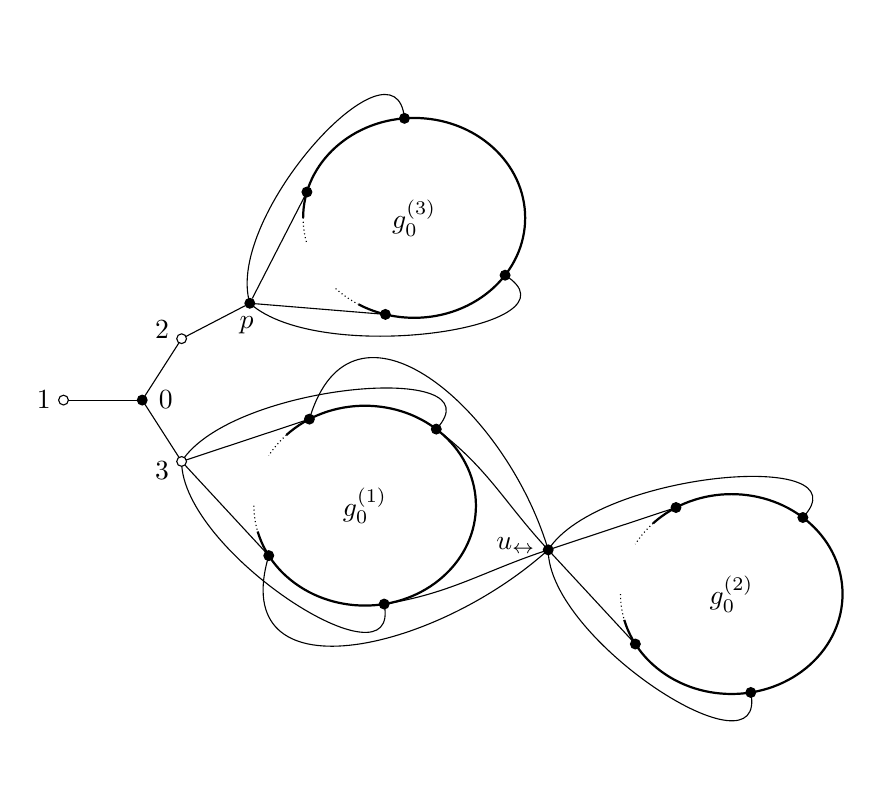
\begin{tikzpicture}[
  yscale = .9,
  label distance=-5.5pt,
  thin,
  vertex/.style={circle,draw=black,fill=black,inner sep=1.25pt,
    minimum size =0mm},
  attach/.style={circle,draw=black,fill=white,inner sep=1.25pt,
    minimum size =0mm},
  dots/.style={circle,fill=black,inner sep=.5pt,
    minimum size= 0pt}]

%%%%%%%%%%%%%%
% G^RT_\leftrightarrow graph
\begin{scope}[yshift=-.866 cm,xshift=.5cm,rotate=255,yshift = 2.41cm]

% Path and Labels    
  
  \node (v) at (0,2.41) [vertex] {};
  \node at (.05,2) {$u_\leftrightarrow$};
  
% Graphs

\foreach \j/\of in {1/0,2/4.82}{
\begin{scope}[yshift=\of cm]
  \foreach \i / \n /\t in {25 / n/ 15, 155 / 1/ 165, 225/ 2 / 120, 315 / {n-1}/60}{

    \node at (\i : 1.41) [vertex] {};
  }
  \node at (0,0) [rectangle,fill=white] {$g_0^{(\j)}$};
  
  \draw[thick] (240:1.41) arc (240:-60:1.41);
  \draw[densely dotted] (240:1.41)  arc (240:255:1.41);
  \draw[densely dotted] (285:1.41)  arc (285:300:1.41);
  
% Attaching Edges
  \foreach \i /\t in {25/15, 155/165}{
    \draw (\i:1.41) to[out=\i,in=\t] (0,-2.41);
  }
  
  \foreach \i \in in {225,315}{
    \draw (\i:1.41) to (0,-2.41);
  }
  
\end{scope}
}

  \draw (25:1.41) to [out = 115,in=-55] (0,2.41);
  \draw (155:1.41) to [out=65,in=-125] (0,2.41);
  \draw[looseness=1.5] (225:1.41) to [out=180,in=210] (0,2.41);
  \draw[looseness=1.5] (315:1.41) to [out=0,in=-30] (0,2.41);

\end{scope}

%%%%%%%%%%%%%%%%%%%%%%%%
% G^RT graph
\begin{scope}[xshift = .5 cm, yshift = .866 cm, rotate = -60, yshift = 3.41 cm]
% Path and Labels    
  
  \node (v) at (0,-2.41) [vertex]{};
  \node at (0.25,-2.6) {$p$};
  \draw (v) -- (0,-3.41); 
  
% Graph  
  \foreach \i / \n /\t in {25 / n/ 15, 155 / 1/ 165, 225/ 2 / 120, 315 / {n-1}/60}{

    \node at (\i : 1.41) [vertex] {};
  }
  \node at (0,0) [rectangle,fill=white] {$g_0^{(3)}$};
  
  \draw[thick] (240:1.41) arc (240:-60:1.41);
  \draw[densely dotted] (240:1.41)  arc (240:255:1.41);
  \draw[densely dotted] (285:1.41)  arc (285:300:1.41);

% Attaching Edges
  \foreach \i /\t in {25/15, 155/165}{
    \draw (\i:1.41) to [out=\i,in=\t] (0,-2.41);
  }
  
  \foreach \i \in in {225,315}{
    \draw (\i:1.41) to (v);
  }
  
\end{scope}

%%%%%%%
% Center stuff
\foreach \t in {60, 180, 300}{
  \draw (0,0) -- (\t:1);
}

\node (0) at (0,0) [vertex] {};
\node (1) at (180:1) [attach] {};
\node (2) at (60:1) [attach]{};
\node (3) at (-60:1) [attach]{};

\node at (0:.3) {$0$};
\node at (-1.25,0) {$1$};
\node at (.25,1) {$2$};
\node at (.25,-1) {$3$};
\end{tikzpicture}
  \caption[Constructed momentum switch]{A momentum switch $\hat G^\prec$ built from a type 2 R/T gadget and its reversal.}
  \label{fig:gen_mom_con}
\end{figure}

We can now prove that this gadget acts as a momentum switch, by constructing the desired scattering eigenstates.

\begin{lemma}\label{lem:mom_switch_construction}
Let $\widehat{G}$ be a type 2 R/T gadget with reflection set $\mathcal{R}$ and transmission set $\mathcal{T}$.  The gadget $\hat{G}^{\prec}$ described above is a momentum switch between the sets $\mathcal{R}$ and $\mathcal{T}$.
\end{lemma}
\begin{proof}

We construct a scattering eigenstate for each momentum $k\in \mathcal{T}$ with perfect transmission from path 1 to path 2, and similarly construct a scattering eigenstate for each momentum $k^{\prime}\in \mathcal{R}$ with perfect transmission from 1 to 3.  These eigenstates show that $S_{2,1}(k) = 1$ and $S_{3,1}(k^\prime) = 1$. Since the S-matrix is symmetric and unitary, this gives the complete form of the S-matrix for all momenta in $\mathcal{R}\cup\mathcal{T}$.  In particular, this shows that $\hat{G}^{\prec}$ is a momentum switch between $\mathcal{R}$ and $\mathcal{T}$.

We first construct the scattering states for momenta $k\in \mathcal{T}$.  \lem{transmit_reqs} shows that the graph $g_0$ has a $2\cos(k)$-eigenvector $\ket{\xi_k}$ satisfying equation \eq{trans_cond} with some nonzero constant $c$. We define a state $\ket{\mu_k}$ on $G^{\prec}$ and we show that it is a scattering eigenstate with perfect transmission between paths $1$ and $2$.   The amplitudes of $\ket{\mu_k}$ on the semi-infinite paths and the claw are
\begin{equation}
  \langle (x,1)|\mu_k\rangle=e^{-ikx} \qquad 
  \langle 0|\mu_k\rangle=1 \qquad 
  \langle (x,2)|\mu_k\rangle=e^{ikx} \qquad
  \langle (x,3)|\mu_k\rangle=0.
\end{equation}
The rest of the graph consists of the three copies of the subgraph $g_0$ and the vertices $p$ and $u_{\leftrightarrow}$. The corresponding amplitudes are
\begin{equation}
  \braket{v}{\mu_k} =
  \begin{cases}
	  -\frac{1}{c}\braket{v}{\xi_k} & v\in V(g^{(1)}_0) \\
    \frac{1}{c}\braket{v}{\xi_k} & v \in V(g^{(2)}_0) \\
	  -\frac{e^{ik}}{c} \braket{v}{\xi_k} & v \in V(g^{(3)}_0) \\
  	0 & v=p \text{ or } v=u_{\leftrightarrow}.
  \end{cases}
\end{equation}

We claim that $\ket{\mu_k}$ is an eigenstate of the Hamiltonian with eigenvalue $2\cos(k)$.  As in previous proofs, the state clearly satisfies the eigenvalue condition on the semi-infinite paths and at the vertices of $G_0$ and $G_0^\leftrightarrow$, and the factors of $\frac{1}{c}$ in the above equation are chosen so that the state also satisfies the eigenvalue condition at vertices $p$ and $u_\leftrightarrow$. Since $\ket{\mu_k}$ is a scattering state with perfect transmission from path 1 to path 2, we see that $S_{2,1}(k) = 1$.

We now construct an eigenstate $\ket{\nu_{k^\prime}}$ with perfect transmission from path 1 to path 3 for each momentum $k^\prime \in \mathcal{R}$.  This state has the form
\begin{equation}
  \langle (x,1)|\nu_{k^\prime}\rangle=e^{-i k^\prime x} \qquad 
  \langle 0|\nu_{k^\prime}\rangle=1 \qquad 
  \langle (x,2)|\nu_{k^\prime}\rangle=0 \qquad
  \langle (x,3)|\nu_{k^\prime}\rangle=e^{i k^\prime x}
\end{equation}
on the semi-infinite paths and the claw.  \lem{reflect_reqs} shows that $G_0$ has a $2\cos(k^\prime)$-eigenstate $\ket{\chi_{k^\prime}}$ with $\braket{p}{\chi_{k'}} \ne 0$, which determines the form of $\ket{\nu_{k^\prime}}$ on the remaining vertices:
\begin{equation}
  \braket{v}{\nu_{k^\prime}} =
  \begin{cases}
	  -\frac{1}{\braket{p}{\chi_{k'}}} \braket{v}{\chi_{k^\prime}} & v \in V(G_0) \\
	  -\frac{e^{ik'}}{\braket{p}{\chi_{k'}}} \braket{v}{\chi_{k^\prime}} & v \in V(g_0^{(2)}) \\
	  -e^{ik'} & v=u^\leftrightarrow \\
    0 & \text{otherwise}.
  \end{cases} 
\end{equation}
As before, it is easy to check that this a momentum-$k^\prime$ scattering state with perfect transmission from path 1 to path 3, so $S_{3,1}(k^\prime)=1$.

Thus the gadget from \fig{gen_mom_con} is a momentum switch between $\mathcal{R}$ and $\mathcal{T}$.
\end{proof}

%%%%%%
\subsubsection{Explicit example}

Using this construction for momentum switches, we can obtain a momentum switch from any of the examples discussed in \sec{rt_ex}.  Explicitly, using the R/T gadget built from the 3-cycle, we get a momentum switch between $-\frac{\pi}{3}$ and $-\frac{2\pi}{3}$, as shown in \fig{mom_switch_ex}.  More generally, using an $r$-cycle, we obtain a switch between momenta of the form $-\frac{\pi j}{r}$ with odd or even values of $j$.  As another example, using a path of length $4$ connected at the center vertex, we obtain a switch between $-\frac{\pi}{4}$ and $-\frac{\pi}{2}$.

\begin{figure}
  \centering
  \tikzsetnextfilename{SG_mom_switch_ex}
  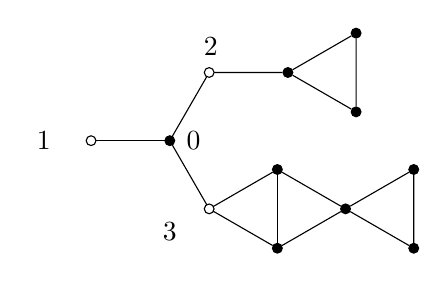
\begin{tikzpicture}[
  label distance=-5.5pt,
  thin,
  vertex/.style={circle,draw=black,fill=black,inner sep=1.25pt,
    minimum size =0mm},
  attach/.style={circle,draw=black,fill=white,inner sep=1.25pt,
    minimum size =0mm},
  dots/.style={circle,fill=black,inner sep=.5pt,
    minimum size= 0pt}]

\begin{scope}[yshift = .866cm, xshift = .5cm,rotate=0]

  \node (b) at (1,0) [vertex] {};
  \node (c) at (1.866,.5) [vertex] {};
  \node (d) at (1.866,-.5) [vertex] {};
  
  \draw (0,0) -- (b) -- (c) -- (d) -- (b);
\end{scope}

\begin{scope}[yshift = -.866cm, xshift = .5cm,rotate= -90]
  \node (e) at (.5,.866) [vertex] {};
  \node (f) at (-.5,.866) [vertex] {};
  \node (g) at (0,1.732) [vertex] {};
  \node (h) at (.5,2.598) [vertex] {};
  \node (i) at (-.5,2.598) [vertex]{};
  
  \draw (0,0) -- (e) -- (g) -- (h) -- (i) -- (g) -- (f) -- (0,0);
  \draw (e) -- (f);

\end{scope}

%%%%%%%
% Center stuff
\foreach \t in {60, 180, 300}{
  \draw (0,0) -- (\t:1);
}

\node (0) at (0,0) [vertex] {};
\node (1) at (180:1) [attach] {};
\node (2) at (60:1) [attach]{};
\node (3) at (-60:1) [attach]{};

\node at (0:.3) {$0$};
\node at (-1.6,0) {$1$};
\node at (0.52,1.2) {$2$};
\node at (0,-1.15) {$3$};

\end{tikzpicture}
  \caption{A momentum switch between $-\frac{\pi}{3}$ and $-\frac{2\pi}{3}$.}
  \label{fig:mom_switch_ex}
\end{figure}


%%%%%%%%%%%%%%%%%%%%%%%%%%%%%%%%%%%%%%
\subsection{Encoded unitaries}\label{sec:gadgets_unitary}

While there is no known efficient method to find graphs that fixed scattering behavior, it is possible to search over all small graphs in order to find gadgets with some particular scattering behavior.  This was the manner in which the gadgets for most known scattering results were found, such as in Childs' original universality proof for graph scattering \cite{Chi09} and Childs, Gosset, and Webb's universality result \cite{MPQW}.  Additionally, Blumer, Underwood, and Feder have a paper \cite{BUF11} in which they searched over all graphs with up to 9 vertices for scattering behavior at particular momentum.

Essentially, the main idea behind this method is a brute force search.  Since we can easily compute the scattering matrix for a particular graph at a particular momentum, if we want to find a graph that has some prescribed scattering behavior, we simply assume that such a graph exists and search for it over all graphs, starting with those having a small number of vertices.  While this exhaustive search is not guaranteed to find such a graph, a surprising number of systems can be found with this structure.  In particular, if we restrict ourselves to momenta that are simple multiples of $\pi$, such as $-\frac{\pi}{2}$ or $-\frac{\pi}{4}$, then most simple scattering behaviors can be found.  

Of particular interest to us will be gadgets with four terminal vertices, such that the scattering matrix at some particular momenta takes the form
\begin{equation}
  S(k) = \begin{pmatrix} 0 & U^T\\
    U & 0\end{pmatrix}. \label{eq:encoded_scat}
\end{equation}
Namely, if we use a dual-rail encoding for a qubit, and think of one pair of semi-infinite paths as the input rails and the other pair as the output rails, then after scattering this gadget will have applied the unitary $U$ to the encoded qubit.

While the general problem is difficult, we might be able to guide our search for specific unitaries.  As a particular example, any one-qubit unitary with a zero-entry will allow us to work with disconnected graphs, and focus on finding a two-terminal gadgets with perfect transmission coefficients.  If we find two such gadgets such that the ratio between their transmission coefficients are the same as the ratio of the entries in the unitary, we can thus implement the unitary.

In the most trivial non-trivial example, we can use this idea to implement an $X$ gate at all momentum by using two length-two paths, where the input terminal for logical $z$ connects to the output terminal of logical $1+z$.  For a slightly less trivial example, note that for any momentum $k$ we can always implement an encoded $\diag\{1,e^{i k}\}$ by using as our graph gadget $\widehat{G}$ a path of length $3$.  Both unitaries are essentially just a relabeling of the vertices, but they are still useful computationally.  


Later in this thesis we will describe a scheme for arbitrary quantum computation using scattering theory as the basic computational tool.  While the scheme makes no reference to a particular momenta, it does require that there are a set of graph gadgets at the correct momenta implementing a universal gate set.  As such, we will want to show that the set of momenta satisfying this assumption is non-empty.

\subsubsection{Universal gate set for $-\frac{\pi}{2}$}

Since the energy corresponding to momentum $-\frac{\pi}{2}$ is zero, the eigenvalue equations for this gadget are slightly easier than average to manipulate.  Additionally, this was the momentum used in \cite{FGG08} in their algorithm for the AND-OR tree.

Note that the the graph in \fig{pi_2_had} and \fig{pi_2_had_planar} both implement a Hadamard gate for a qubit encoded at momentum $-\frac{\pi}{2}$, but that the graph in \fig{pi_2_had_planar} is planar.  In particular, \fig{pi_2_had} has a scattering matrix of the form \eq{encoded_scat}, with
\begin{equation}
  U = -\frac{e^{i \frac{\pi}{4}}}{\sqrt{2}}\begin{pmatrix}
    1 & 1\\
    1 & -1 
  \end{pmatrix}, 
\end{equation}  
while \fig{pi_2_had_planar} implements


\begin{figure}
  \centering
  \subfloat[][]{ 
    \tikzsetnextfilename{SG_pi_2_had}
    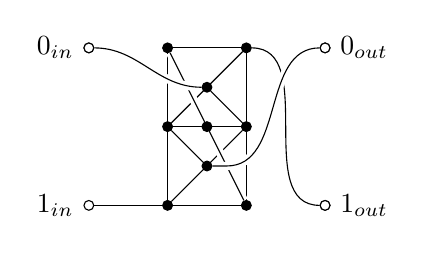
\begin{tikzpicture}
  [ scale=1,
    thin,
    attach/.style={circle,fill=white,draw=black,
      inner sep=1.25pt,minimum size=0pt},
    vert/.style={circle,draw=black,fill=black,
      inner sep=1.25pt,minimum size=0pt}]
  
    \node (0inhad) at (0,2) [attach]{};
    \node (1inhad) at (0,0) [attach]{};
    \node (0outhad) at (3,2) [attach]{};
    \node (1outhad) at (3,0) [attach]{};
    
    \node (1had) at (1,0) [vert]{};
    \node (2had) at (2,0) [vert]{};
    \node (3had) at (1.5,.5) [vert]{};
    \node (4had) at (1,1) [vert]{};
    \node (5had) at (1.5,1) [vert] {};
    \node (6had) at (2,1) [vert] {};
    \node (7had) at (1.5,1.5) [vert]{};
    \node (8had) at (1,2) [vert]{};
    \node (9had) at (2,2) [vert]{};

    \draw (8had) -- (1had);
    \draw (9had) -- (2had);
    \draw (4had) -- (9had);
    \draw (1had) -- (6had);
    \draw (4had) -- (6had);
    \draw (3had) -- (4had);
    \draw (7had) -- (6had);
    \draw (1inhad) -- (2had);
    \draw (8had) -- (9had);
    \draw (8had) -- (5had)[line width=3pt,white];
    \draw (5had) -- (2had)[line width=3pt,white];
    \draw (8had) -- (2had);
    
    \draw (9had) to[out=0,in=180] (1outhad) [looseness=.3];
    \draw (0inhad) to[out=0,in=180] (7had)[line width = 3pt,white];
    \draw (0inhad) to[out=0,in=180] (7had);

    \draw (3had) --(1.75,.5) to[out=0,in=180] (0outhad)[line width =3pt,white];
    \draw (3had) --(1.75,.5) to[out=0,in=180] (0outhad);

    \node at (0inhad) [attach]{};
    \node at (1outhad) [attach]{};
    \node at (0outhad) [attach]{};


  \node at (1inhad.west) [left] {$1_{\text{in}}$};
  \node at (0inhad.west) [left] {$0_{\text{in}}$};
  \node at (0outhad.east) [right] {$0_{\text{out}}$};
  \node at (1outhad.east) [right] {$1_{\text{out}}$};
\end{tikzpicture}
    \label{fig:pi_2_had}
  }
  \qquad
  \subfloat[][]{
    \tikzsetnextfilename{SG_pi_2_had_planar}
    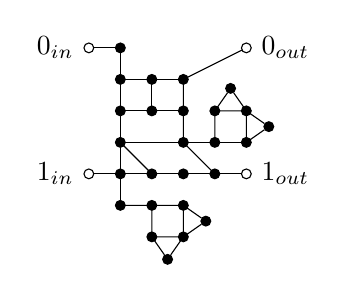
\begin{tikzpicture}
  [ scale = .4,
  	thin,
    inner/.style={circle,draw=black!100,fill=black!100,inner sep = 1.25pt},
    attach/.style={circle,draw=black!100,fill=black!0,thin,inner sep=1.25pt},
    cross/.style={draw=white,double=black,thin}]

 \node at (0,0)[inner] {};
 \node at (1,0)[inner] {};
 \node at (2,0)[inner] {};
 \node at (0,1)[inner] {};
 \node at (2,1)[inner] {};
 \node at (0,2)[inner] {};
 \node at (1,2)[inner] {};
 \node at (2,2)[inner] {};
 \node at (0,3)[inner] {};
 \node at (1,3)[inner] {};
 \node at (2,3)[inner] {};
 \node at (3,1)[inner]{};
 \node at (4,1)[inner]{};
 \node at (3,2)[inner]{};
 \node at (4,2)[inner]{};
 \node at (3,0)[inner]{};
 \node (a) at (3.5,2.714)[inner]{};
 \node (b) at (4.714,1.5)[inner]{};
 \node at (0,-1) [inner]{};
 \node at (1,-1) [inner]{};
 \node at (2,-1) [inner]{};
 \node at (1,-2) [inner]{};
 \node at (2,-2) [inner]{};
 \node (c) at (2.714,-1.5) [inner]{};
 \node (d) at (1.5,-2.714) [inner]{};
 \node at (0,4) [inner]{};

 \draw (-1,0) -- (4,0);
 \draw (-1,4) -- (0,4);
 \draw (0,4) -- (0,-1);
 \draw (0,2) -- (2,2);
 \draw (0,3) -- (2,3);
 \draw (0,1) -- (4,1);
 \draw (1,3) -- (1,2);
 \draw (3,0) -- (2,1) -- (2,3);
 \draw (0,1) -- (1,0);
 \draw (2,3) -- (4,4);
 
 \draw (0,-1) -- (2,-1) -- (c) -- (2,-2) -- (2,-1);
 \draw (1,-1) -- (1,-2) -- (2,-2) -- (d) -- (1,-2);
 
 \draw (4,1) -- (b) -- (4,2) -- (4,1);
 \draw (3,1) -- (3,2) -- (a) -- (4,2) -- (3,2);

 \node at (-1,0) [attach,label=left:$1_{\text{in}}$]{};
 \node at (-1,4) [attach,label=left:$0_{\text{in}}$]{};
 \node at (4,4) [attach,label=right:$0_{\text{out}}$]{};
 \node at (4,0) [attach,label=right:$1_{\text{out}}$]{};
 
\end{tikzpicture}
    \label{fig:pi_2_had_planar}
   }
  \caption[Hadamard gadget at $\frac{\pi}{2}$]{Two gates that implement an encoded Hadamard at $-\frac{\pi}{4}$.  \subfig{pi_2_had}  A simple gate.  \subfig{pi_2_had_planar}  More complicated but planar gate.}
   \label{fig:pi_2_universal}
\end{figure}




If we then combine this unitary with the $\diag\{e^{-i\pi/2}\}$ gate that works for all unitaries, we then have that we can implement all single-qubit Clifford gates.  Thus in order to have a universal set of single-qubit gates we simply need to find a single unitary not contained within the Clifford group.


As such an example, we can use the diagonal graph depicted in \fig{pi_2_nonClifford}.  This is related to the $V$-basis often used for fault-tolerant computations, where the implemented unitary is 
\begin{equation}
  U = \begin{pmatrix}
    1 & 0\\
    0 &  \frac{4 - 3 i}{5}
  \end{pmatrix}. 
\end{equation}  

%%%%%%%%%%%%%%%%%
\begin{figure}
  \centering
  \tikzsetnextfilename{SG_pi_2_nonClifford}
  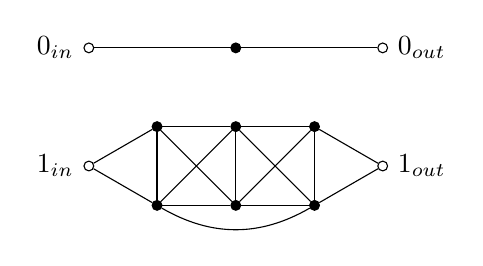
\begin{tikzpicture}
  [inner/.style={circle,draw=black!100,fill=black!100,inner sep = 1.25pt},
    attach/.style={circle,draw=black!100,fill=black!0,thin,inner sep = 1.25pt}]

  \node (0in) at (-1.866, 2) [attach, label=left:$0_{\text{in}}$] {};
  \node (0out) at (1.866, 2) [attach, label=right:$0_{\text{out}}$] {};
  \node at (0,2) [inner] {};

  \node (1) at (-1.866, .5) [attach, label=left:$1_{\text{in}}$] {};
  \node (2) at (1.866, .5) [attach, label=right:$1_{\text{out}}$] {};
  \node (3) at (-1      , 1) [inner] {};
  \node (4) at ( 0, 1) [inner] {};
  \node (5) at ( 1, 1) [inner] {};
  \node (6) at (-1, 0) [inner] {};
  \node (7) at (0 , 0) [inner] {};
  \node (8) at (1 , 0) [inner] {};

  \draw (0in) to (0out) [thin];

  \draw (1) to (3) [thin];
  \draw (1) to (6) [thin];
  \draw (2) to (5) [thin];
  \draw (2) to (8) [thin];
  \draw (3) to (4) [thin];
  \draw (3) to (6) [thin];
  \draw (3) to (7) [thin];
  \draw (4) to (5) [thin];
  \draw (4) to (6) [thin];
  \draw (4) to (7) [thin];
  \draw (4) to (8) [thin];
  \draw (5) to (7) [thin];
  \draw (5) to (8) [thin];
  \draw (6) to (7) [thin];
  \draw (7) to (8) [thin];
  \draw (6) to[out=330,in=210] (8) [thin];

\end{tikzpicture}
  \caption[Non-clifford gadget at $\frac{\pi}{2}$]{Graph implementing a non-Clifford gate at $k = -\frac{\pi}{2}$.
    \label{fig:pi_2_nonClifford}}
\end{figure}



\subsubsection{Universal gate set for $-\frac{\pi}{4}$}

Historically \cite{Chi09,MPQW}, momentum $-\frac{\pi}{4}$ has been used to show universality results.  I'm unsure why, except that the graph gadgets that implement a universal gate set are rather simple at this momenta.  

In particular, Childs found that the two gadgets in \fig{pi_4_universal} implement a universal gate set.  His original proof required some additional attributes on the graph gadgets, which is the reason for the slightly more complicated $T$-gate, but this is sufficient for our purposes.

%%%%%%%%%%%%%%%%%%%%%%%%%%%%
\begin{figure}
  \centering
  \subfloat[][]{ 
    \tikzsetnextfilename{SG_pi_4_phase}
    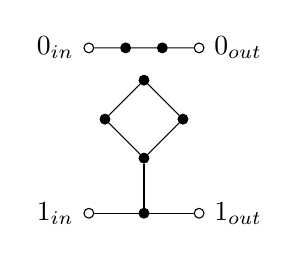
\begin{tikzpicture}
  [ scale=0.7,inner/.style={circle,draw=black!100,fill=black!100,inner sep = 1.25pt},
    attach/.style={circle,draw=black!100,fill=black!0,thin,inner sep = 1.25pt}]
  \node (0) at (-1,      0)      [attach,label=left:$1_\text{in}$] {};
  \node (1) at ( 0,      0)      [inner]  {};
  \node (2) at ( 1,      0)      [attach,label=right:$1_\text{out}$] {};  
  \node (3) at ( 0,      1)      [inner]  {};
  \node (4) at ( 0,      2.4142) [inner]  {};
  \node (5) at (-0.7071, 1.7071) [inner]  {};
  \node (6) at ( 0.7071, 1.7071) [inner]  {};
  \node (7) at (-1,      3)      [attach,label=left:$0_\text{in}$] {};
  \node (8) at (-0.3333, 3)      [inner]  {};
  \node (9) at ( 0.3333, 3)      [inner]  {};
  \node (10)at ( 1,      3)      [attach,label=right:$0_\text{out}$] {};

  \draw (1) to (0) [thin];
  \draw (1) to (2) [thin];
  \draw (1) to (3) [thin];
  \draw (3) to (5) [thin];
  \draw (3) to (6) [thin];
  \draw (5) to (4) [thin];
  \draw (6) to (4) [thin];  
  \draw (8) to (7) [thin];
  \draw (8) to (9) [thin];
  \draw (9) to (10)[thin];
\end{tikzpicture}
    \label{fig:pi_4_phase}
  }
  \qquad
  \subfloat[][]{
    \tikzsetnextfilename{SG_pi_4_basis_change}
    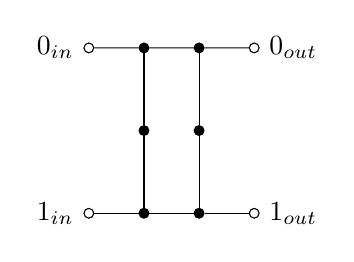
\begin{tikzpicture}
  [ scale=0.7,
    yscale=1.5,
    inner/.style={circle,draw=black!100,fill=black!100,inner sep = 1.25pt},
    attach/.style={circle,draw=black!100,fill=black!0,thin,inner sep = 1.25pt}]

  \node (1) at ( 0, 2) [inner]  {};
  \node (2) at ( 0, 0) [inner]  {};
  \node (3) at ( 1, 2) [inner]  {};
  \node (4) at ( 1, 0) [inner]  {};
  \node (5) at ( 0, 1) [inner]  {};
  \node (6) at ( 1, 1) [inner]  {};
  \node (7) at (-1, 2) [attach,label=left:$0_\text{in}$] {};
  \node (8) at (-1, 0) [attach,label=left:$1_\text{in}$] {};
  \node (9) at ( 2, 2) [attach,label=right:$0_{\text{out}}$] {};
  \node (0) at ( 2, 0) [attach,label=right:$1_{\text{out}}$] {};

  \draw (7) to (1) [thin];
  \draw (8) to (2) [thin];
  \draw (3) to (9) [thin];
  \draw (4) to (0) [thin];
  \draw (1) to (3) [thin];
  \draw (1) to (5) [thin];
  \draw (2) to (4) [thin];
  \draw (2) to (5) [thin];
  \draw (3) to (6) [thin];
  \draw (4) to (6) [thin];
\end{tikzpicture}
    \label{fig:pi_4_basis_change}
   }
   \caption[Universal gadget set at $\frac{\pi}{4}$]{Encoded one-qubit gates at $k = -\frac{\pi}{4}$.  \subfig{pi_4_phase}  A phase gate.  \subfig{pi_4_basis_change}  Basis-changing gate.}
   \label{fig:pi_4_universal}
\end{figure}


In particular, we have that the graph in \fig{pi_4_phase} has a scattering matrix of the form of equation \eq{encoded_scat} at momentum $k= -\frac{\pi}{4}$, with 
\begin{equation}
  U = \begin{pmatrix}
    e^{- i \frac{\pi}{4}} & 0\\
    0 & 1 
  \end{pmatrix},
\end{equation}
while the gadget in \fig{pi_4_basis_change} also has a scattering matrix of the form \eq{encoded_scat} at momentum $k=-\frac{\pi}{4}$, where
\begin{equation}
  U = -\frac{i}{\sqrt{2}}\begin{pmatrix}
    1 & -i\\
    -i & 1 
  \end{pmatrix}.
\end{equation}



With these examples, we then have a universal gate set for single-qubit unitaries at $-\frac{\pi}{4}$, which will be sufficient for our eventual purposes.  

\subsubsection{Universal gate set at $-\frac{\pi}{3}$ and $-\frac{2\pi}{3}$}

While the previous two momenta are relevant for historical reasons, we would also like to show a universal gate set at other momentum.  By looking forward in the thesis, where we will be interested in two momenta moving along adjacent paths, it will be useful to have the two wave-functions move at the same speed, and thus will be interesting to study $k$ and $-\pi - k$ for some $k\in (-\pi,0)$.  A natural choice would be then to understand $-\frac{\pi}{3}$ and $-\frac{2\pi}{3}$, since they are nicely separated, and further we have an explicit momentum switch between the two momenta.

Unfortunately, most gadgets in the Blumer, et. al., database for these two momenta are related to $e^{-i \pi/3}$, whereas most Clifford gates are related to $e^{i \pi/4}$, and thus we unfortunately don't know of a set of gadgets implementing a Clifford+T-gate set.  However, there are sufficient graphs in order to have a universal set, but it is one note widely used.

In particular, note that the simple shifted diagonal gadget described in the beginning of this section allows us to implement a $\diag\{1,e^{2i \pi/3}\}$ gate for both momenta of interest.  In addition to this single gadget, the graph in \fig{pi_3_universal} implements another gate, corresponding to a rotation along a different axis on the Bloch sphere.  

\begin{figure}
  \centering
  \tikzsetnextfilename{SG_pi_3_universal}
  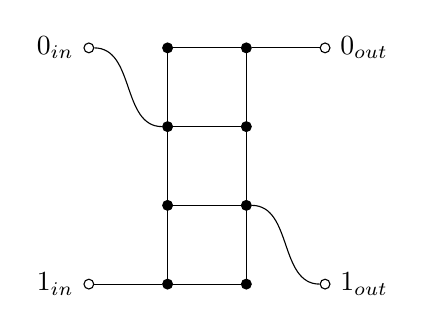
\begin{tikzpicture}
  [inner/.style={circle,draw=black!100,fill=black!100,inner sep = 1.25pt},
    attach/.style={circle,draw=black!100,fill=black!0,thin,inner sep = 1.25pt}]
    
  \node (2) at (-1,0) [attach, label=left:$1_\text{in}$] {};
  \node (9) at (0,0) [inner] {};
  \node (10) at (0,2) [inner] {};
  \node (11) at (1,3) [inner] {};
  \node (12) at (1,1) [inner] {};
  \node (8) at (1,0) [inner] {};
  \node (7) at (0,1) [inner] {};
  \node (4) at (2,0) [attach,label=right:$1_\text{out}$] {};
  \node (1) at (-1,3) [attach,label=left:$0_\text{in}$] {};
  \node (6) at (1,2) [inner] {};
  \node (5) at (0,3) [inner] {};
  \node (3) at (2,3) [attach, label=right:$0_\text{out}$] {};

  \draw (5) to (9) [thin];
  \draw (5) to (11) [thin];
  \draw (9) to (8) [thin];
  \draw (11) to (8) [thin];
  \draw (10) to (6) [thin];
  \draw (7) to (12) [thin];
  \draw (1) to[out = 0, in=180] (10) [thin];
  \draw (2) to (9) [thin];
  \draw (3) to (11) [thin];
  \draw (4) to[out =180, in=0] (12) [thin];
\end{tikzpicture}
  \caption[Non-clifford gadget at $\frac{\pi}{3}$ and $\frac{2\pi}{3}$]{A non-clifford gate used for universal computation at $-\frac{\pi}{3}$ and $-\frac{2\pi}{3}$.}
  \label{fig:pi_3_universal}
\end{figure}

The graph in \fig{pi_3_universal} has an $S$-matrix with perfect transmission at both momenta of interest, with the corresponding unitary given by
\begin{align}
  U(-\frac{\pi}{3}) &= \frac{e^{5i \pi/6}}{2} \begin{pmatrix}
    \sqrt{3} & e^{ i \pi/6}\\
    e^{- i \pi/6} & \sqrt{3}
  \end{pmatrix} &
  U(-\frac{2\pi}{3}) &=  \frac{e^{-5i \pi/6}}{2} \begin{pmatrix}
    \sqrt{3} & e^{- i \pi/6}\\
    e^{ i \pi/6} & \sqrt{3}
  \end{pmatrix}
\end{align}


%%%%%%%%%%%%%%%%%%%%%%%%%%%%%%%%%%%%%%%%%%%%%%%%%%%%%%%%%%%%%%%%%

%%%%%%%%%%%%%%%%%%%%%%%%%%%%%%%%%%%%%%%%%%%%%%%%%%%%%%%%%%%%%%%%%
\section{Sufficient and disallowed scattering behavior}

While the previous constructions yield graphs with particular behavior which will be useful when attempting to construct scattering algorithms, we will also want to understand some simple relations between graphs and their respective scattering matrices.  In particular, understanding what properties are necessary in order to have a given scattering matrix, and understanding the relation between various the scattering matrices of various momenta will be useful in constructing additional scattering graphs.

\subsection{Degree-3 graphs are sufficient}

One of the most simple assumptions that could be made is that certain scattering behaviors require high degree graphs.  In particular, having many connections might allow for additional correlations between outputs on larger graphs.  

If we restrict our attention to a finite number of rational momenta, however, this does not turn out to be the case.  We can show that any graph can be replaced by a degree-three graph with a identical scattering behavior at some fixed momenta.  In particular, we will show that a single vertex can be replaced by a finite path while still satisfying the eigenvalue equation at the fixed momenta, where the length of the path is dependent on the fixed momenta.

As degree two graphs are the graph joins of cycles and paths, degree three graphs are the smallest graphs to have nontrivial scattering behaviors.  This lemma shows that, in a certain sense, they are also all that are required.

\begin{lemma} Let $\widehat{G}$ be a finite graph, and let $M$ be a finite set of rational multiples of $\pi$.  If $v\in V(G)$ is a degree $d$ vertex, there exists a graph $H$ that extends $G$ with the vertex $v$ being replaced by a degree-$(\lceil \frac{d}{2}\rceil +1)$ subgraph such that the scattering matrices at the momenta $k\in M$ are preserved.
\label{lem:degree_reduction}
\end{lemma}
\begin{proof}
  The main idea behind this proof is to partition the vertices adjacent to $v$ into two sets, and then replace $v$ by a finite path, with the two sets connected to opposites ends of the finite path.  By choosing the length of the path correctly, we can show that the amplitudes at either end of the path are the same as the amplitude on $v$ at each momenta in $M$, and thus the eigenvalue equation remains satisfied without changing the scattering behavior.  
  
  In particular, let $v$ be the degree $d$ vertex in $G$, and let $S = \{w\in V(G) : w\sim v\}$ be the set of vertices adjacent to $v$.  Additionally, let us arbitrarily partition $S$ into two sets, $S_1$ and $S_2$, such that $\big||S_1|-|S_2|\big| \leq 1$.
  
  As each $k\in M$ is a rational multiple of $\pi$, there exists some $m\in \NN^+$ such that $\frac{mk}{2\pi} \in \NN$ for all $k\in M$.  Let us then examine the graph $H$ where $v$ is replaced by a path of length $m$, and where $S_1$ is attached to one end of the path while $S_2$ is attached to the other end.  Explicitly:
  \begin{align}
    V(H) &= \big(V(G)\setminus \{v\}\big) \cup \{(v,j): j\in [m+1]\}\\
    E(H) &= \big\{ e\in E(G) : v\notin e\big\} \cup \big\{ \{(v,j),(v,j+1)\} : j\in [m]\big\} \cup \nonumber\\
    &\qquad \big\{ \{s, (v,0)\} : s\in S_1\big\} \cup \big\{ \{s,(v,m)\} : s\in S_2\big\}.
  \end{align}
  
  Now, for any $k\in M$, let $\ket{\phi}$ be an eigenstate of $A(G)$ with eigenvalue $2\cos(k)$.  We will show that there exists an eigenstate $\ket{\psi}$ of $A(H)$ with energy $2\cos(k)$ such that for any $w\in V(G)\setminus \{v\}$, $\braket{w}{\phi} = \braket{w}{\psi}$.  
  
  Concretely, for any vertex other than $v$, let us define $\ket{\psi}$ in this manner, and note that by assumption, $\ket{\psi}$ satisfies the eigenvalue equation with energy $2\cos(k)$ for all vertices other than those in $S$ or those replacing $v$.  Additionally, let 
  \begin{equation}
    \alpha = \sum_{w\in S_1} \braket{w}{\phi}, \qquad \beta = \braket{v}{\phi}, \qquad \text{ and } \qquad \gamma = \sum_{w\in S_2} \braket{w}{\phi}.
  \end{equation}
  We will then defined the amplitude along the path replacing the vertex $v$ as
  \begin{equation}
    \braket{(v,j)}{\psi} = \beta \cos(k j) + \frac{\gamma - \beta\cos(k)}{\sin(k)} \sin( k j).
  \end{equation}
  Note that $\braket{(v,0)}{\psi} = \braket{(v,m)}{\psi} = \beta = \braket{v}{\phi}$, and thus the eigenvalue equation is satisfied at all vertices in $S$.  As the eigenstates along a path with energy $2\cos(k)$ are scalar multiples of $\sin(k x)$ and $\cos(k j)$, we can also see that the eigenvalue equation is necessarily satisfied for all $(v,j)$ with $j\neq 0$ and $j\neq m$.
  
  If we then examine the eigenvalue equation at $(v,0)$, we can see that
  \begin{align}
    \sum_{s\in S_1} \braket{s}{\psi} + \braket{(v,1)}{\psi} &= \alpha + \beta \cos(k) + \frac{\gamma - \beta \cos(k)}{\sin(k)} \sin (k) \\
      &= \alpha + \gamma \\
      &= 2 \cos(k) \beta = 2 \cos(k) \braket{(v,0)}{\psi}
  \end{align}
  where the third equality follows from the fact that $\ket{\phi}$ satisfies the eigenvalue equation at $v$ with eigenvalue $2\cos(k)$, and thus we have that the eigenvalue equation for $H$ is satisfied at $(v,0)$. 
  
  Let us finally examine the eigenvalue equation at $(v,m)$, noting that
  \begin{align}
    \sum_{s\in S_2} \braket{s}{\psi} + \braket{(v,m-1)}{\psi} &=\gamma + \beta \cos(k (m-1)) + \frac{\gamma - \beta \cos(k)}{\sin(k)} \sin (k(m-1)) \\
      &= \gamma + \beta \cos(k)   -  \big(\gamma - \beta \cos(k)\big)\\
      &= 2 \cos(k) \beta = 2 \cos(k) \braket{(v,0)}{\psi}
  \end{align}
  where the second equality follows from some trigonometric identities. We can then see that $\ket{\psi}$ satisfies the eigenvalue equation at $(v,m)$ with energy $2\cos(k)$.
  
  Putting this together, we have that $\ket{\psi}$ is an eigenvector of $A(H)$ with energy $2\cos(k)$ such that $\ket{\psi}$ and $\ket{\phi}$ are identical on those vertices contained in both $G$ and $H$.  As this result holds for any energy $2\cos(k)$ eigenvector of $A(G)$, and as the two graphs are identical along the semi-inifinite paths, we have that the scattering states for these two graphs are identical, and thus the scattering matrices are preserved under this degree reduction procedure.
\end{proof}

By repeated use of this lemma, we can then reduce any graph used as a scattering gadget down to a degree-3 graph without changing the scattering matrix at some fixed momentum.


%%%%%%%%%%%%%%%%%%%%%%%%%%%%%%%%%%%%%%%%%%%%%%%%%%%%%%%%%%%%%%%%%

\subsection{Some behavior impossible}

So far, all of our constructions have generally assumed that the scattering behavior that we want does exist.  Hence, if we simply search over large enough graphs, we will eventually find a graph that implements our desired scattering behavior.

However, it turns out that in some cases this is not a valid assumption.  In particular, there exist pairs of momenta for which no R/T gadget can be constructed.  The main idea is that for specific momentum, there exists a basis for the scattering states in which all amplitudes are taken from a field extension of the rationals.  If two momenta are related by a Galois conjugation over this field, then perfect reflection at one momenta implies perfect reflection at the second.  Note that this is a result in \cite{MomSwitches}.

As an illuminating example, we will use those states with momenta $k= -\frac{\pi}{4}$ and $p = - \frac{3\pi}{4}$.  For the two momenta, the corresponding energy is $2 \sqrt{2}$ or $-2\sqrt{2}$, and in this case the Galois conjugation is simply replacing $\sqrt{2}$ by $-\sqrt{2}$. 


\subsubsection{Basis vectors with entries in $\QQ(\sin(k),\cos(k))$}
\label{sec:vecs_over_field}

Recall the general setup shown in \fig{basic_graph}: $N$ semi-infinite paths are attached to a finite graph $\widehat G$, resulting in an infinite graph $G$.  Additionally, we have that the adjacency matrix for $\widehat{G}$ can be written in block diagonal form
\begin{align}
  A(\widehat{G}) = \begin{pmatrix} 
    A & B^\dag\\
    B & D
  \end{pmatrix},
\end{align}
where $A$ is an $N\times N$ matrix, $B$ is an $m\times N$ matrix, and $D$ is an $m\times m$ matrix.  We have that the $N$ semi-infinite paths are attached, in order, to the first $N$ vertices of $\widehat{G}$.

Let us now consider an eigenvector $\ket{\tau_k}$ of the adjacency matrix of $G$ with eigenvalue $2\cos(k)$ for $k\in (-\pi,0)$.  We have from \thm{scat_basis} that this eigenspace is spanned by incoming scattering states with momentum $k$ and confined bound states (which have zero amplitude on the semi-infinite paths) . We can thus write the amplitudes of $\ket{\tau_k}$ on the semi-infinite paths as
\begin{equation}
  \braket{(x,j)}{\tau_k} 
  = \kappa_j \cos(k (x-1)) + \sigma_j \sin(k (x-1))
\end{equation}
for $x \in \posint$, $j \in [N]$, and $\kappa_j,\sigma_j \in \CC$, and the amplitudes on the internal vertices as
\begin{equation}
  \braket{w}{\tau_k} = \iota_w
\end{equation}
for $\iota_w \in \CC$, where $w$ indexes the internal vertices.  Since the state $\ket{\tau_k}$ satisfies the eigenvalue equation on the semi-infinite paths, it remains to satisfy the conditions specified by the block matrix equation
\begin{equation*}
  \begin{pmatrix} A & B^\dag\\ B & D\end{pmatrix}
	\begin{pmatrix} \kappa \\ \iota \end{pmatrix}
	+ \cos(k) \begin{pmatrix} \kappa \\ 0 \end{pmatrix}
	+ \sin(k) \begin{pmatrix} \sigma \\ 0 \end{pmatrix} 
	= 2\cos(k) \begin{pmatrix} \kappa \\ \iota \end{pmatrix}.
\end{equation*}

Hence, the nullspace of the matrix
\begin{equation}
  M= \begin{pmatrix} A -\cos(k) \II & \sin(k) \II & B^\dag\\
    0 & 0 & 0\\
    B & 0 & D-2\cos(k)\II\end{pmatrix}
\end{equation}
is in one-to-one correspondence with the $2\cos(k)$-eigenspace of the infinite matrix (here the first block corresponds to $\kappa$, the second to $\sigma$, and the third to $\iota$). Further, $M$ only has entries in $\QQ(\cos(k),\sin(k))$, so its nullspace has a basis with amplitudes in $\QQ(\cos(k),\sin(k))$, as can be seen using Gaussian elimination.

We can then use this, along with the form of the eigenstates along the semi-infinite paths, to see that all of the amplitudes can be written as elements over the rationals extended by $\sin(nk)$ and $\cos(nk)$ for all $n\in \NN^+$.  While this is not particularly useful in general, if $k$ is a rational multiple of $\pi$, this is a finite extension.  Further, there exist special cases in which this field extension is a quadratic extension, such that all of the amplitudes can be taken from $\QQ[\sqrt{d}]$ for some $d$.

As a slight caveat noted above, the spectrum of $G$ may include confined bound states (\thm{scat_basis}) with eigenvalues at $2\cos(k)$.  However, any such state is also in the nullspace of the matrix $M$, while also satisfying the rational constraints that both $\kappa$ and $\sigma$ are zero.  As such, these states can always be written with amplitudes over the field $\QQ[\sin(k),\cos(k)]$.  Thus forcing the scattering eigenstates to be orthogonal to these confined bound states only involves constraints over the same field, and we still have that the scattering eigenstates can be written with all of their amplitudes over the field $\QQ$ extended by $\sin(nk)$ and $\cos(nk)$.

As an explicit example, let us examine the case where $2\cos(k)=\pm\sqrt{2}$ corresponding to $k = -\frac{\pi}{4}$ or $k = -\frac{3\pi}{4}$.  In these cases $\QQ(\cos(k),\sin(k)) = \QQ(\sqrt{2})$, and we may choose a basis for the nullspace of $M$ with amplitudes from $\QQ(\sqrt{2})$. Furthermore, $\cos(kx), \sin(kx) \in \QQ(\sqrt{2})$ for all $x\in \posint$, so with such a choice of basis, each amplitude of $\ket{\tau_k}$ is also an element of $\QQ(\sqrt{2})$.

We can then use the fact that $\QQ[\sqrt{2}]$ can be thought of as a two-dimensional vectorspace over $\QQ$ to see that any member of this extended rational basis can be written as 
\begin{align}
  \ket{\tau_k} = \ket{u_k} + \sqrt{2} \ket{w_k},
\end{align}
for rational vectors $\ket{u_k}$ and $\ket{w_k}$.  Further, as $H^2 \ket{\tau_k} = 2 \ket{\tau_k}$, we can see that  $H\ket{u_k}=\pm 2\ket{w_k}$ and $H\ket{w_k} = \pm \ket{u_k}$, so
\begin{equation}
  \ket{\tau_k}=(H \pm \sqrt{2} \II)\ket{w_k},\label{eq:form_of_tau}
\end{equation}
where the $\pm$ depends on whether we are working with $k = -\frac{\pi}{4}$ or $-\frac{3\pi}{4}$.

While this expression does not easily generalize to most pairs of momenta, we do have a similar equation whenever the extended field is a quadratic extension, where $2$ replaced with $d$.


%================================================================
\subsubsection{Impossibility of R/T gadgets}

With the above rational basis for scattering states, we will be able to transform an eigenstate at one energy into an eigenstate at another energy via a Galois conjugation.  However, the existence of particular eigenstates will not immediately give us the results that we want. 

Along these lines, we will use the following basic fact about two-terminal gadgets several times: 
\begin{fact}\label{fct:zero_ampl}
If a two-terminal gadget has a momentum-$k$ scattering state $\ket{\phi}$ with zero amplitude along path $2$, then the gadget perfectly reflects at momentum $k$.
\end{fact}
\begin{proof}
Without loss of generality, we may assume that $\ket{\phi}$ is orthogonal to all confined bound states.
If $\ket{\phi}$ has zero amplitude along path $2$, then there exist some $\mu,\nu \in \CC$ such that
\begin{equation}
  \braket{(x,2)}{\phi}
  = \mu \braket{(x,2)}{\scat_2 (k)} + \nu \braket{(x,2)}{\scat_1(k)}
  = \mu e^{-ikx} + \mu R e^{ikx} + \nu T e^{ikx}
  = 0
\end{equation} 
for all $x\in \ZZ^{+}$.  Since this holds for all $x$, we have $\mu = \mu R + \nu T = 0$.  Since $\mu$ and $\nu$ cannot both be zero, we have $T=0$.
\end{proof}

For an R/T gadget, the scattering states (at some fixed momentum) that are orthogonal to the confined bound states span a two-dimensional space. As shown in \sec{vecs_over_field}, we can expand each scattering eigenstate over an extension to the field $\QQ$.  Let us restrict our attention to the case where this extension is quadratic, with discriminant $d$.

In particular, let us assume that the scattering state at $k$ has energy $\sqrt{d}$ (with $d$ nonsquare) and can be written in a basis with entries over $\QQ(\sqrt{d})$, where each basis vector takes the form \eq{form_of_tau}. This gives
\begin{equation*}
  \ket{\scat_{1}(k)} 
  = (H + \sqrt{d}\II) (\alpha \ket{a} + \beta \ket{b}) \label{eq:rat_expansion}
\end{equation*}
where $\alpha,\beta \in \CC$, $\alpha\neq 0$, and $\ket{a}$ and $\ket{b}$ are rational $d$-eigenvectors of $H^2$.

If $T(k) = 0$, then for all $x \geq 0$, 
\begin{equation}
  \langle x,2\ket{\scat_1(k)} 
  = 0 
  = \langle{x,2} |(H + \sqrt{d}\II) (\alpha \ket{a} + \beta \ket{b}).
\end{equation}
Dividing through by $\alpha$ and rearranging, we get that for all $x\geq 0$,
\begin{equation*}
\frac{\beta}{\alpha} (\langle{x,2}| H\ket{b}+\sqrt{d} \langle{x,2}\ket{b})
  =-\langle{x,2}| H\ket{a}  -\sqrt{d} \langle{x,2}\ket{a}.
\label{eq:cases_eqn}
\end{equation*}
If the left-hand side is not zero, then $\beta/\alpha \in \QQ(\sqrt{d})$ since $H$, $\ket{a}$, and $\ket{b}$ are rational.  If the left-hand side is zero, then $(H+ \sqrt{d}\II)\ket{a}$ is an eigenstate at energy $2\cos(k)$ with no amplitude along path 2, so $\beta = 0$ (using \fct{zero_ampl}), and again $\beta/\alpha \in \QQ(\sqrt{d})$.

Now write $\beta/\alpha=r+s\sqrt{d}$ with $r,s\in\QQ$, and consider the rational $d$-eigenvector of $H^2$
\begin{equation}
  \ket{c} := \ket{a} + (r+sH) \ket{b}.
\end{equation}
Note that
\begin{equation}
  \alpha (H + \sqrt{d} \II) \ket{c} 
= \alpha(H+ \sqrt{d} \II) \ket{a} + \alpha (rH+r\sqrt{d}+ sH^2+sH\sqrt{d}) \ket{b}.
\end{equation}
Since $\ket{b}$ is a $d$-eigenvector of $H^2$ and $\beta/\alpha=r+s\sqrt{d}$, this simplifies to
\begin{equation}
  \alpha (H + \sqrt{d}\II) \ket{c} 
  = \alpha (H + \sqrt{d}\II) \ket{a} + \beta(H + \sqrt{d}\II) \ket{b} 
  = \ket{\scat_1(k)}, \label{eq:sc1_c}
\end{equation}
so $\ket{\scat_1(k)}$ can be written as $\alpha(H+\sqrt{d}\II)$ times a rational $d$-eigenvector of $H^2$.

Since $\langle{x,2}\ket{\scat_1(k)} = 0$ for all $x\geq 1$ (and $\alpha\neq 0$), we have
\begin{equation}
  \langle{x,2}| (H+\sqrt{d}\II) \ket{c} 
  = \langle{x,2}| H \ket{c} + \sqrt{d} \langle{x,2}\ket{c} 
  = 0.
\end{equation}
As $H$ is a rational matrix and $\ket{c}$ is a rational vector, the rational and irrational components must both be zero, implying $\langle{x,2}\ket{c}  =\langle{x,2}|H\ket{c} = 0$ for all $x\geq 1$. Furthermore, since $ \ket{\scat_1(k)}$ is a scattering state with zero amplitude on path $2$, it must have some nonzero amplitude on path 1 and thus there is some $x_0\in \mathbb{Z}^+$ for which $\langle{x_0,1}\ket{c}\neq 0$ or $\langle{x_0,1}|H\ket{c} \neq 0$.

Now consider the state obtained by replacing $\sqrt{d}$ with $-\sqrt{d}$, or in other words after performing a Galois conjugation:
\begin{equation}
  \ket{\overline{\scat}_1(k)} := \alpha (H-\sqrt{d}\II) \ket{c}.
\end{equation}
This is a $-\sqrt{d}$-eigenvector of $H$, which can be confirmed using the fact that $\ket{c}$ is a $d$-eigenvector of $H^2$. As $\langle{x,2} | H \ket{c} = \langle x,2 \ket{c} = 0$ for all $x\geq 1$, $\langle x,2 \ket{\overline{\scat}_1(k)} = 0$ for all $x\geq 1$. Furthermore the amplitude at vertex $(x_0,1)$ is nonzero, i.e.,  $\langle x_0,1 \ket{\overline{\scat}_1(k)} \neq 0$, and hence $\ket{\overline{\scat}_1(k)}$ has a component orthogonal to the space of confined bound states (which have zero amplitude on both semi-infinite paths).  Hence, there exists a scattering state with eigenvalue $-\sqrt{d}$ with no amplitude on path 2. By \fct{zero_ampl}, the gadget perfectly reflects at momentum $p$, where $p = -\pi - k$ corresponds to this energy.  It follows that no perfect R/T gadget (and hence no perfect momentum switch) exists between these momenta.

As particular cases, we can take $k = -\frac{\pi}{4}$, where $d = 2$.  In this case, we have that there does not exist an $R/T$ gadget splitting $k$ and $-\frac{3\pi}{4}$.   Similarly, it is possible to show that $k = -\frac{\pi}{6}$ can be written in a basis with entries over $\QQ[\sqrt{3}]$, and thus there does not exist a R/T gadget between $k$ and $-\frac{5\pi}{6}$. 

%\subsubsection{Approximate R/T gadget}
%
%\todo{I never particularly liked this bit, and I'll think I'll include it later if I have the time}
%
%
%%%%%%%%%%%%%%%%%%%%
%\subsection{Laplacians vs adjacency matrix}
%
%\todo{If I have time, write this section.  The basic idea is similar to proof removing self-loops from the graph for the BH model.  In particular, in order to turn a degree 3 graph into a 3-regular graph, we use three copies of the original graph.  For each degree-2 vertex $u$ in the original graph, we add another vertex $u_0$ to the overall graph, and add edges from all three $u_i$ for $i\in[3]$ to $u_0$.  For each degree-1 vertex, we do this twice.  Note that for each eigenstate of the original graph, there are two with nearly the same amplitudes.  We can then use these for our scattering eigenstates}
%




%%%%%%%%%%%%%%%%%%%%%%%%%%%%%%%%
\section{Conclusions and extensions}

At this point, we have a large number of graph gadgets that each implement different scattering behavior.  We have found several sets of gadgets that implement universal sets of single-qubit gates at particular momentum, and we can construct momentum switches between many different momenta.  

Additionally, we have also shown that some scattering behavior cannot exist.  While this means that certain schemes cannot be simplified, this result is of independent theoretical interest.  Further, it also allows us to stop searching for graphs with these behaviors.  It would be interesting to extend our results on the impossibility, however, and give a large set of disallowed scattering behaviors.

While these form a nice foundation, more research can always be done in these fields.  Ideally, giving an explicit algorithm that constructs a graph with a particular scattering behavior, or says that such a graph doesn't exist, would be of great interest.  Even if such an algorithm took an exponential amount of time, this would be a theoretical achievement since we don't know whether this problem is currently decidable.  Less ambitiously, if we could construct such an algorithm for a restricted set of graphs, such as that given for type 1 and type 2 R/T gadgets, but generalized to multiple input and outputs, we would be very useful for computations involving graph scattering.  

\biblio{}

\end{document}
